% Section content template for individual Educative lessons
% This file contains the actual content for a specific section
% Generated from Educative API section content

% Section: System Design: The Sharded Counters
% Section ID: 6071347163955200
% Section Slug: system-design-the-sharded-counters
% Generated: 2025-12-07T22:16:12.383643

\subsection{Problem statement}\label{KEimBjItKXWsquUiFIuKV}
\\
Real-time applications like Facebook, Twitter, and YouTube have high user traffic. Users interact with the applications and perform multiple operations (view, like, comment, and so on) depending on the application's structure. For instance, an image is posted on a Facebook page that has millions of followers, and the post's likes rapidly increase after each millisecond. Here, it might be easy to count the likes for this single image, but what will we do when thousands of such images or videos are uploaded simultaneously by many celebrities, each with millions of followers. This problem is known as the \textbf{heavy hitters problem}.
\\
The above scenario shows how a simple counting operation becomes challenging to manage with precision and performance. The following figure shows YouTube's videos that were viewed by millions of users in a 24-hour span in August 2021:

\begin{figure}[htbp]
 \centering
 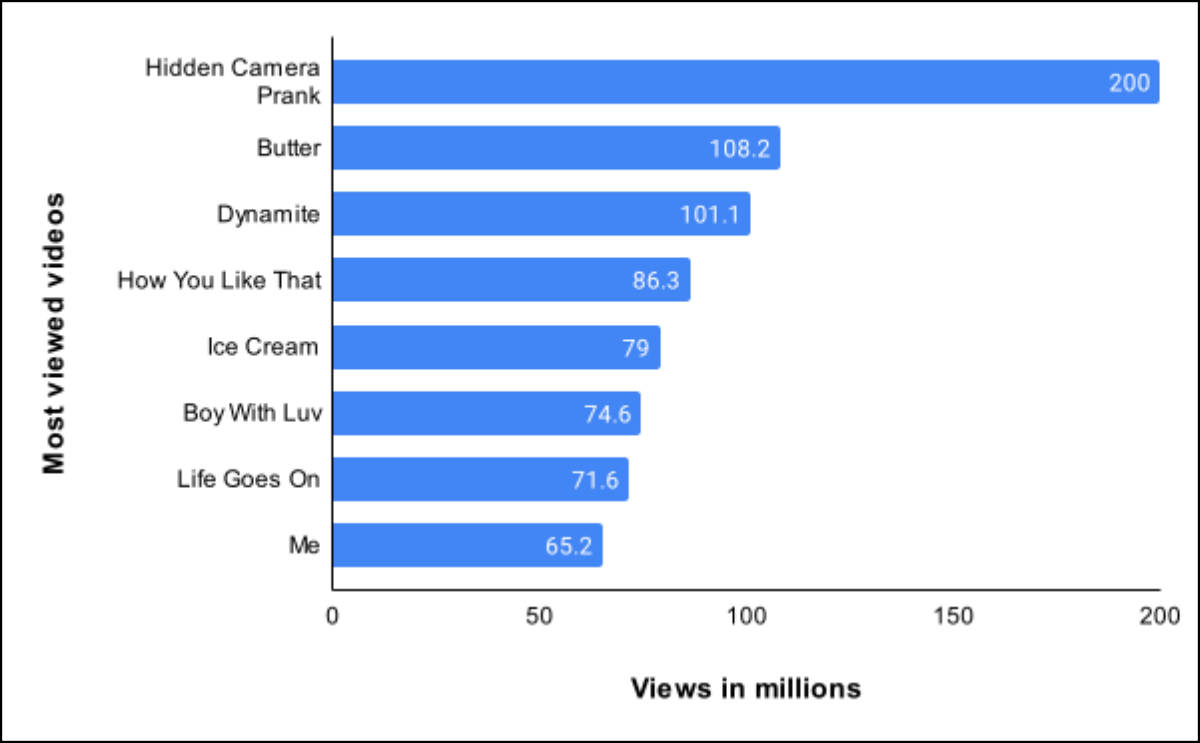
\includegraphics[width=0.5\textwidth]{Images/chapter_24/section_6071347163955200/6383174573883392.png}
 \caption{YouTube videos' views in 24 hours}
\end{figure}

On average, six thousand tweets are sent on Twitter within one second, which equals 360,000 tweets per minute and about 500 million tweets per day. A challenging task is to handle billions of likes on these 500 million tweets per day. The following table shows the most liked tweets in one day as of 2022:\\

\begin{figure}[htbp]
 \centering
 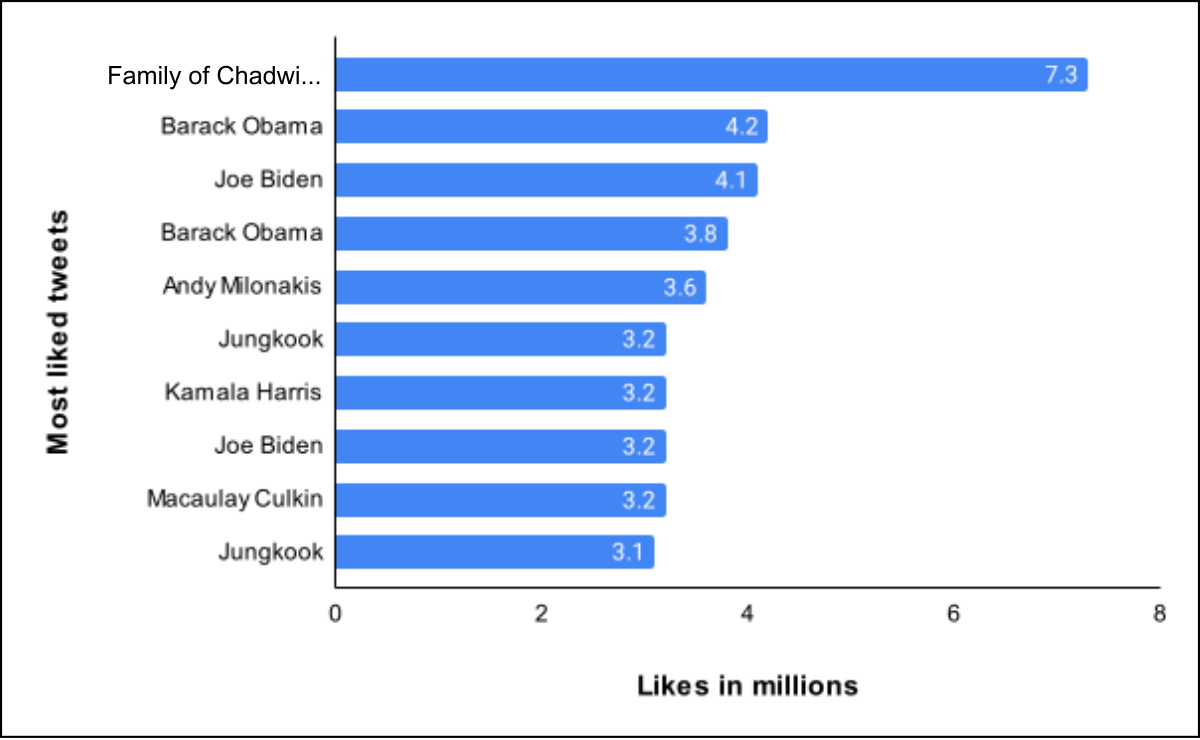
\includegraphics[width=0.5\textwidth]{Images/chapter_24/section_6071347163955200/5015212726157312.png}
 \caption{Most liked tweets in a single day}
\end{figure}

How will we handle millions of write requests coming against the likes on thousands of tweets per minute? The challenge is that writing takes more time than reading, and concurrent activity makes this problem harder. As the number of concurrent writes increases for some counter (which might be a variable residing in a node\textquotesingle s memory), the lock contention increases non-linearly. After some point, we might spend most of the time acquiring the lock so that we could safely update the counter.\\

\subsection{How will we design sharded counters?}\label{N-EkheN-U1odqVLEweXY6}
\\
We have divided the design of sharded counters into three lessons:

\begin{enumerate}
\item
\protect\phantomsection\label{FxgYIV72obpF0-nXG4q_8}
\href{https://www.educative.io/courses/grokking-the-system-design-interview/high-level-design-of-sharded-counters}{\textbf{High-level Design}}: We'll discuss the high-level design of sharded counters in this lesson. In addition, we'll also briefly explain the API design.
\item
\protect\phantomsection\label{-Wm6XUbkoh6i7PKPBFbpo}
\href{https://www.educative.io/courses/grokking-the-system-design-interview/detailed-design-of-sharded-counters}{\textbf{Detailed Design}}: This lesson will dive deeply into the design of sharded counters. Moreover, we'll also evaluate our proposed design.
\item
\protect\phantomsection\label{woU9fW54ixB_O86f5Sl6g}
\href{https://www.educative.io/courses/grokking-the-system-design-interview/quiz-on-the-sharded-counters-design}{\textbf{Quiz}}: We'll review major concepts of sharded counters design with a quiz.
\end{enumerate}
\\
Let's begin with the high-level solution sketch of sharded counters.

% End of section content